\begin{frame}[allowframebreaks]{Laufzeitmessung}
    \begin{figure}
        \centering
        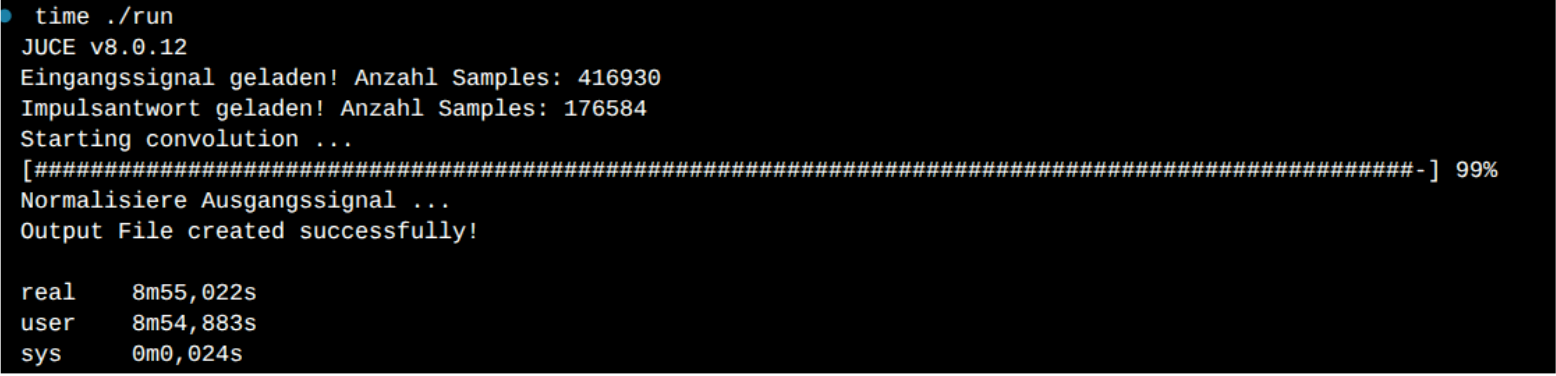
\includegraphics[width=0.8\textwidth]{Graphics/runtime_measurement.png}
        \caption{Messung des gezeigten Codes \ref{fig:cpp_code} unter Verwendung des Linux-Tools \textit{time}}
    \end{figure}
    \begin{itemize}
        \item Samplerate beider Signale: 44100 Hz
        \item Eingangssignal: Etwa 10-sekündiges Gitarrensignal
        \item Impulsantwort: Etwa 5 Sekunden
        \item Laufzeitklasse: $\mathcal{O}(N \cdot M)$ (vgl. Folie \ref{frame:runtime_analysis})
    \end{itemize}
    \framebreak
    \begin{itemize}
        \item Anzahl der Berechnungen für das $\approx$ 15-sekündige Ausgangssignal:
    \end{itemize}
    \begin{equation}
        \begin{split}
            G_{Berechnungen} &= (N + M - 1) \cdot M \\
                            &= (416.930 + 176.584 - 1) \cdot 176.584 = 104.804.899.592 \\
        \end{split}
    \end{equation}
    \begin{itemize}
    \item Entspricht $\approx$ 7-Milliarden Berechnungen, die der Prozessor in einer Echtzeitanwendung ausführen müsste.
    \end{itemize}
\end{frame}
